\RequirePackage{fix-cm}
%
\RequirePackage{amsmath}



%\documentclass{svjour3}                     % onecolumn (standard format)
%\documentclass[smallcondensed]{svjour3}     % onecolumn (ditto)
%\documentclass[smallextended]{svjour3}       % onecolumn (second format)
% \documentclass[twocolumn]{svjour3}          % twocolumn
%\documentclass[letterpaper, 12pt, twocolumn]{article}
\documentclass{article}
\usepackage[cm]{fullpage}
%\usepackage[margin=1in]{geometry}
\usepackage{amssymb}
\usepackage{graphicx}
\usepackage[utf8]{inputenc}
\usepackage{indentfirst}
%\usepackage{physics}
\newcommand{\me}{\mathrm{e}}
\usepackage{amsmath}
\usepackage{varwidth}
\usepackage[binary-units]{siunitx}
\usepackage{algpseudocode}
\usepackage{circuitikz}


%\usepackage[monochrome]{color}

%\usepackage[round]{natbib}
%\usepackage{apacite}
\usepackage{url}


\PassOptionsToPackage{monochrome}{xcolor}

% For the flow charts
\usepackage{tikz}
\usetikzlibrary{
	external,
}
%\tikzexternalize

\usetikzlibrary{shapes.geometric, arrows, calc, positioning}
\tikzstyle{startstop} = [rectangle, thick, rounded corners=2.5mm, minimum width=2cm, minimum height=5mm,text centered, draw=black]
\tikzstyle{io} = [trapezium, thick, trapezium left angle=70, trapezium right angle=110, text width=3.75cm, minimum height=0.5cm, text centered, draw=black]
\tikzstyle{process} = [rectangle, thick, minimum width=2.5cm, text width=4cm, minimum height=0.5cm, text centered, draw=black]
\tikzstyle{block} = [rectangle, thick, minimum width=0.5cm, minimum height=1cm, text centered, draw=black]
\tikzstyle{support} = [coordinate, join=by fuzzy]
\tikzstyle{decision} = [diamond, thick, minimum width=3cm, minimum height=1cm, text centered, draw=black]
\tikzstyle{dottedbox} = [rectangle, dotted, thick, minimum width=2.5cm, text width=2.8cm, minimum height=0.5cm, text centered, draw=black]
\tikzstyle{arrow} = [thick,->,>=stealth]
\tikzstyle{dottedarrow} = [thick, dotted,->,>=stealth]





\usepackage{pgfplots}
\usepgfplotslibrary{patchplots}
\pgfplotsset{compat=newest, samples=015} %Set this value to 65 for the final version
%\usepgfplotslibrary{dateplot} 


%\providecommand{\keywords}[1]{\textbf{\textit{Index terms---}} #1}

%\journalname{Journal of Science Education and Technology}

\begin{document}
\section{Tables}
\begin{table}
	\centering
	\caption{Characteristics of bridge circuit used by the authors}
	\label{Tab:BridgeCharacteristics}
	\begin{tabular}{|p{5cm}|l|}
		\hline
		\textbf{Property}     & \textbf{Value} \\ \hline
		Analog input voltage range         & \SIrange{0}{5}{\volt} \\ \hline
		Analog input resolution &  1024 \\ \hline
		Analog output type & PWM\\ \hline
		Analog output voltage range         & \SIrange{0}{5}{\volt} \\ \hline
		Analog output resolution &  256 \\ \hline
		Baud rate for RS232 protocol & \SI{115200}{\bit\per\second}\\ \hline
	\end{tabular}
\end{table}

\section{Figures}
\begin{figure}
	\begin{tikzpicture}[node distance = 10mm, auto]
	\node (Excitation) [align=center] {
	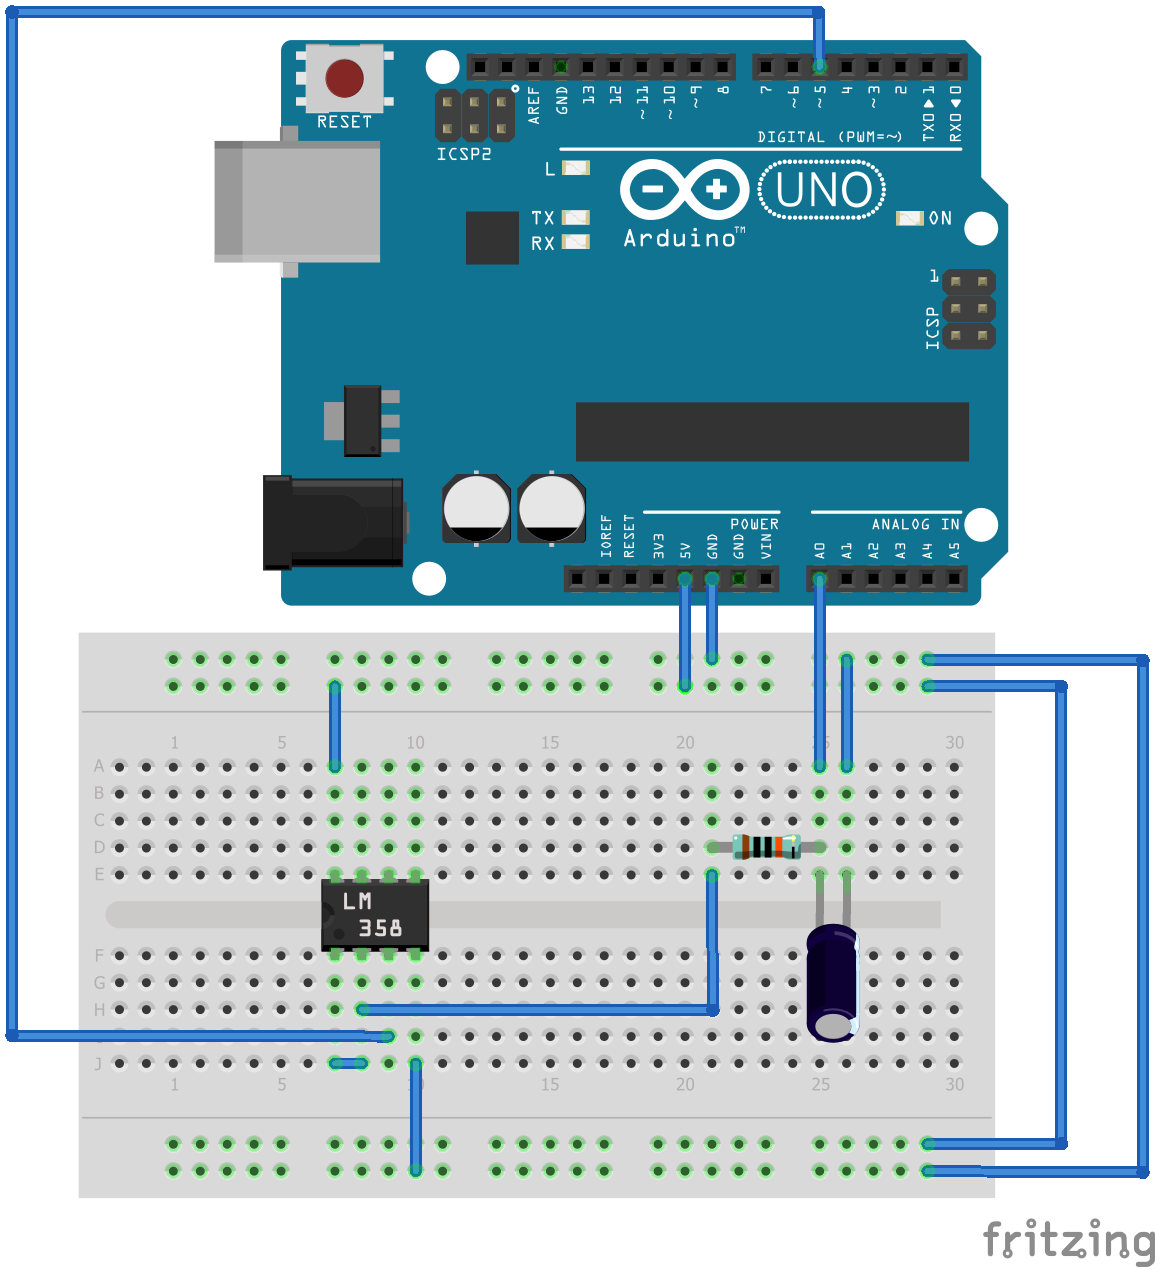
\includegraphics[scale=1]{images/bridge-circuit.png}
	};
	\end{tikzpicture}

	
	\caption{Bridge and RC circuit}
	\label{Fig:BridgeCircuit}
\end{figure}


\begin{figure}
	\centering
	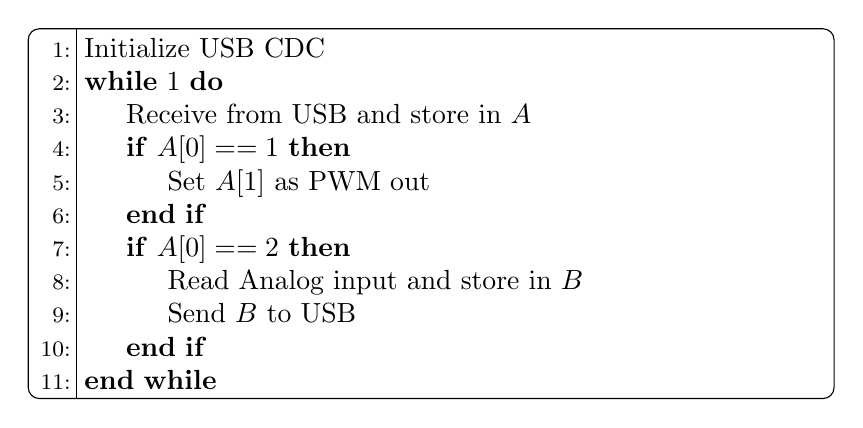
\begin{tikzpicture}[node distance = 10mm, auto]
	\node (algorithm) [draw, rounded corners, text width = 10cm] {% 
		\begin{varwidth}{\linewidth}
		\begin{algorithmic}[1]
		\State Initialize USB CDC
		\While {1}
		\State Receive from USB and store in $A$
		\If{$A[0]==1$}
		\State Set $A[1]$ as PWM out
		\EndIf
		\If{$A[0]==2$}
		\State Read Analog input and store in $B$
		\State Send $B$ to USB
		\EndIf
		\EndWhile
		\end{algorithmic}
		\end{varwidth}
		%
	};
	\draw [-] (algorithm.north)+(-45mm, 0) -- (-45mm,1mm);
	\draw [-] (algorithm.south)+(-45mm, 0) -- (-45mm, 1mm);
	\end{tikzpicture}
	\caption{Bridge device's firmware}
	\label{Fig:Firmware}
\end{figure}

\begin{figure}
	\centering
	\begin{tikzpicture}[node distance = 10mm, auto]
	\node (Excitation) [align=center] {
		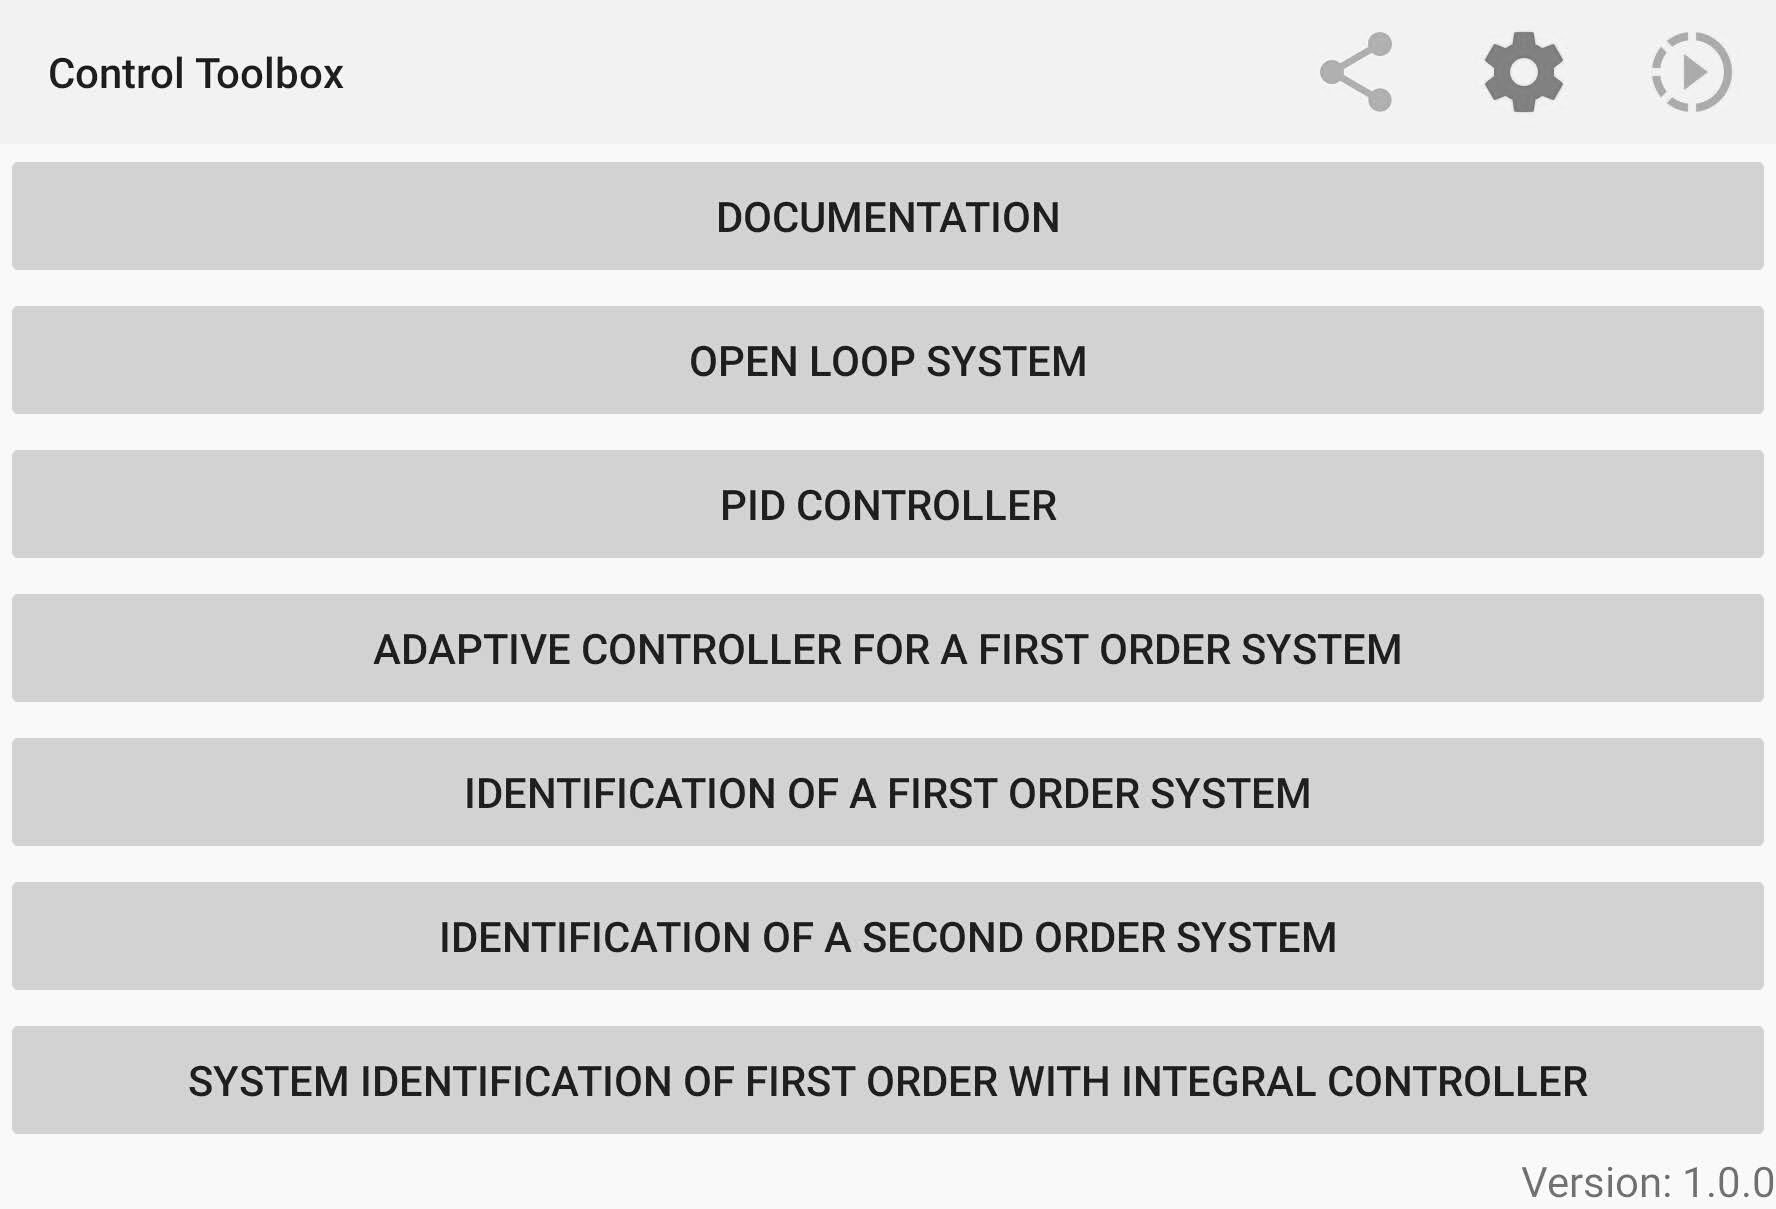
\includegraphics[width=0.49\textwidth]{images/home-screen.jpg}
	};
	\end{tikzpicture}
	\caption{Android App home screen}
	\label{Fig:HomeScreen}
\end{figure}

\begin{figure}
	\centering
	\begin{tikzpicture}[node distance = 10mm, auto]
	\node (Excitation) [align=center] {
		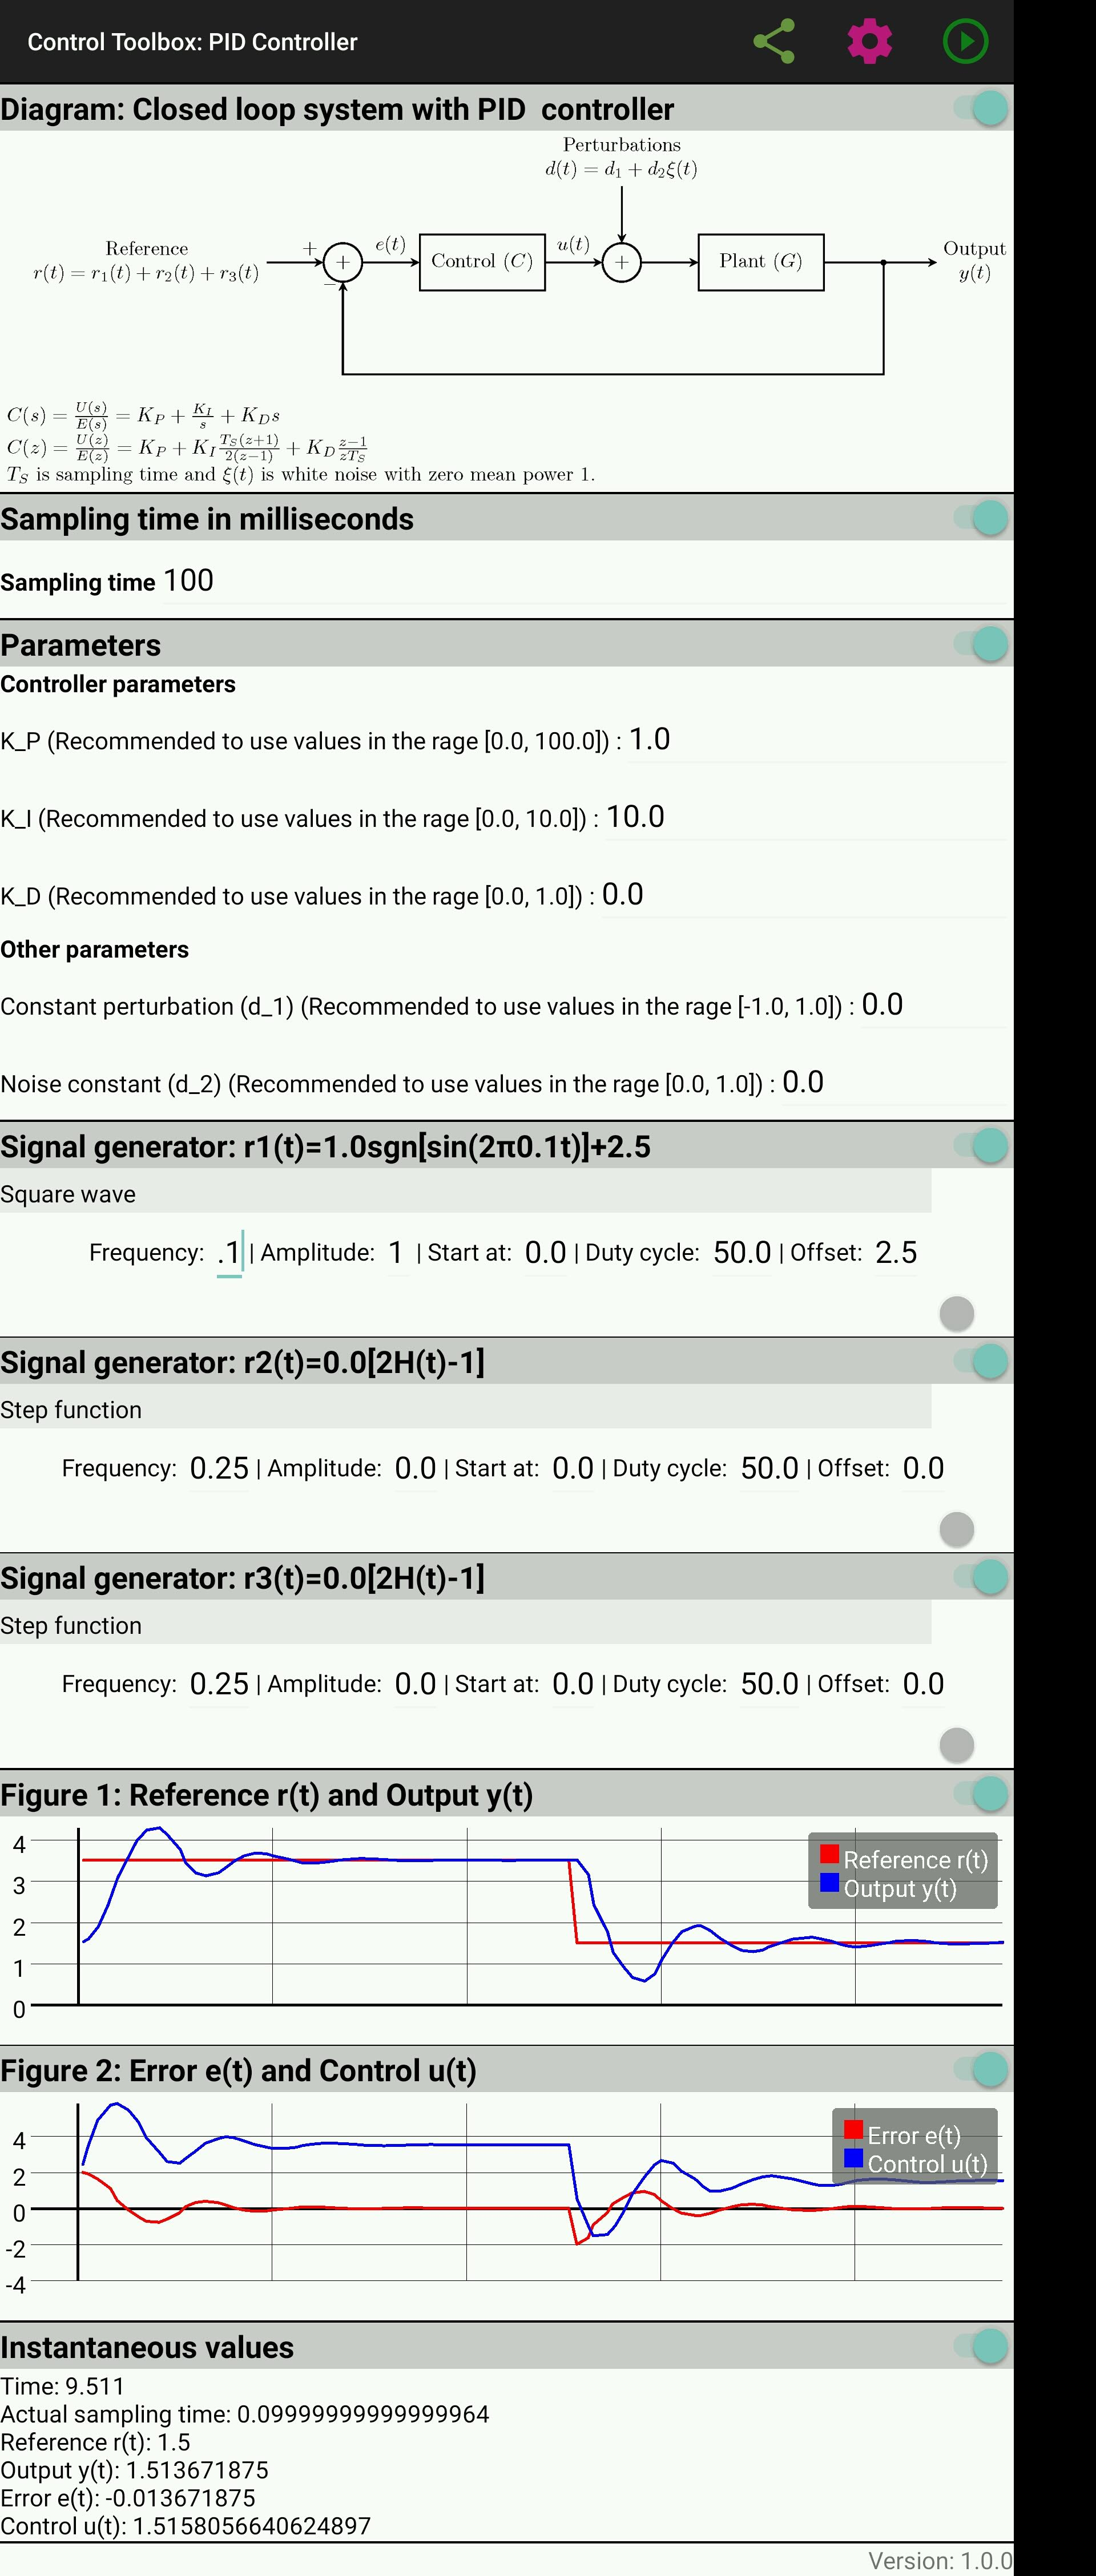
\includegraphics[width=0.49\textwidth]{images/pid-control-screen.jpg}
	};
	\end{tikzpicture}
	\caption{Android App running closed loop control system with PID controller when bridge circuit is connected to a low pass filter }
	\label{Fig:PIDView}
\end{figure}

\begin{figure}
	\centering
	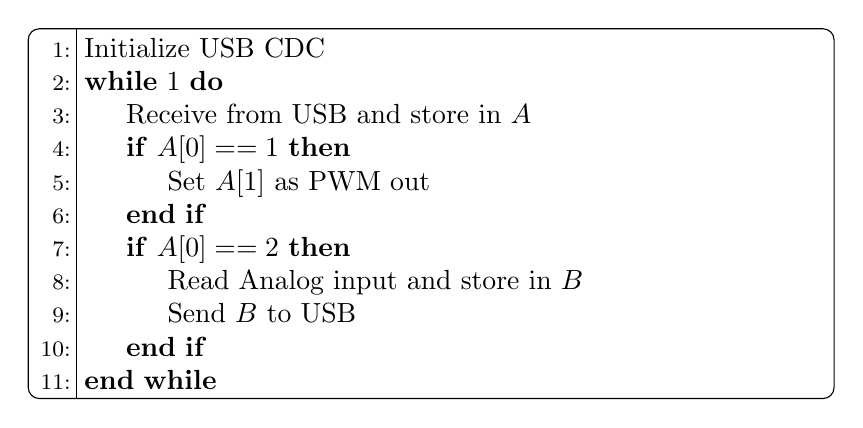
\begin{tikzpicture}[node distance = 10mm, auto]
	\node (algorithm) [draw, rounded corners, text width = 10cm] {% 
		\begin{varwidth}{\linewidth}
		\begin{algorithmic}[1]
		\State Initialize USB CDC
		\While {1}
		\State Receive from USB and store in $A$
		\If{$A[0]==1$}
		\State Set $A[1]$ as PWM out
		\EndIf
		\If{$A[0]==2$}
		\State Read Analog input and store in $B$
		\State Send $B$ to USB
		\EndIf
		\EndWhile
		\end{algorithmic}
		\end{varwidth}
		%
	};
	\draw [-] (algorithm.north)+(-45mm, 0) -- (-45mm,1mm);
	\draw [-] (algorithm.south)+(-45mm, 0) -- (-45mm, 1mm);
	\end{tikzpicture}
	\caption{Android app implementation of the real-time algorithm}
	\label{Fig:RealTimeAlgorithm}
\end{figure}

\begin{figure}
	\centering
	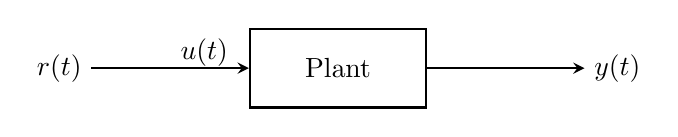
\begin{tikzpicture}[node distance = 10mm, auto]
	\node (Input) [align=center] {$r(t)$};
	\node (Plant) [block, text width = 2cm, right = 2cm of Input] {Plant};
	\node (Output) [right = of Plant, right = 2cm, align=center] {$y(t)$};
	\draw [arrow] (Input) -- node[above = 2mm, anchor= west	]{$u(t)$}(Plant);
	\draw [arrow] (Plant) -- (Output);
	\end{tikzpicture}
	\caption{Open loop system}
	\label{Fig:BlockDiagramOpenLoop}
\end{figure}

\begin{figure}
	\centering
	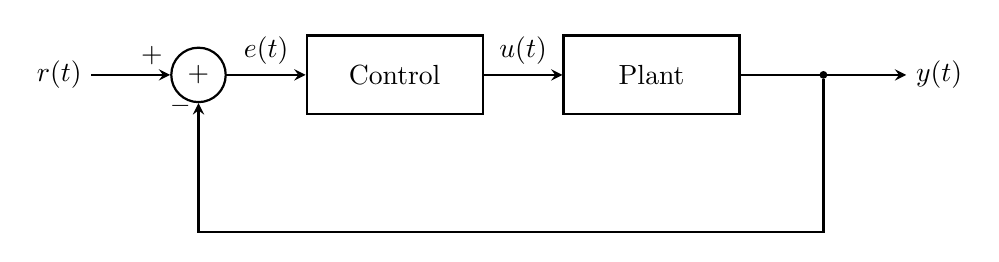
\begin{tikzpicture}[node distance = 10mm, auto]
	\node (Reference) [align=center] {$r(t)$};
	\node (SummingPoint) [draw,circle, thick, right = of Reference]  {+};
	\node (Control) [block, text width = 2cm, right = of SummingPoint] {Control};
	\node (Plant) [block, text width = 2cm, right = of Control] {Plant};
	\node (PlantRight) [support, right = of Plant, fill, circle,scale=0.3] {};
	\node (Output) [right = of PlantRight,  align=center] {$y(t)$};
	\draw [arrow] (Reference) -- node[anchor=south west]{+}(SummingPoint);
	\draw [arrow] (SummingPoint) -- node[anchor=south]{$e(t)$}(Control);
	\draw [arrow] (Control) -- node[anchor=south]{$u(t)$}(Plant);
	\draw [arrow] (Plant) -- (Output);
	\draw [arrow] (PlantRight) -- +(0, -2) -| (SummingPoint) node[below = 2mm, anchor=north east]{\bf\textendash};
	\end{tikzpicture}
	\caption{Closed loop system}
	\label{Fig:BlockDiagramClosedLoop}
\end{figure}

\begin{figure}
	\centering
	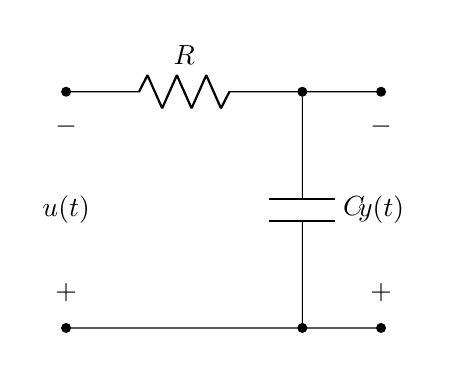
\begin{tikzpicture}[node distance = 10mm, auto]
	\node (Excitation) [align=center] {
		\begin{circuitikz}[american][americanvoltages]
		\draw (0,0)
		to [open, -*, v^>=$u(t)$] (0,3) 
		to[R, -*, l=$R$] (3,3)
		to[C, -*, l=$C$] (3,0)
		to[short, -*] (0,0);
		\draw (3,3)
		to [short, -*] (4,3)
		to [open, -*, v^<=$y(t)$] (4,0)
		to [short] (3,0);
%		\draw[thin, <-, >=triangle 45] (1,1)node{$i_1$}  ++(-60:0.5) arc (-60:170:0.5);		
		\end{circuitikz}
	};
	\end{tikzpicture}
	\caption{First order low pass filter}
	\label{Fig:CircuitRC1}
\end{figure}

\begin{figure}
	\centering
	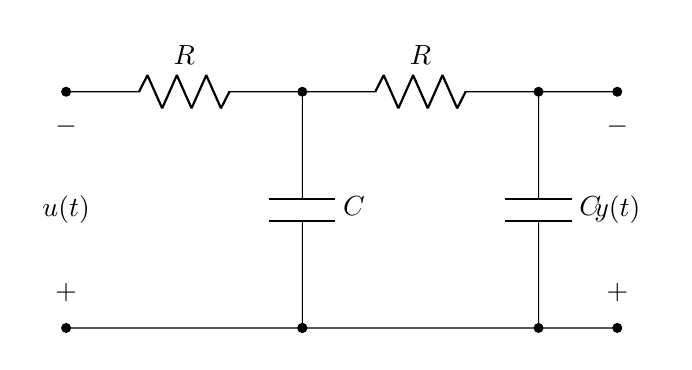
\begin{tikzpicture}[node distance = 10mm, auto]
	\node (Excitation) [align=center] {
		\begin{circuitikz}[american][americanvoltages]
		\draw (0,0)
		to [open, -*, v^>=$u(t)$] (0,3) 
		to[R, -*, l=$R$] (3,3)
		to[C, -*, l=$C$] (3,0)
		to[short, -*] (0,0);
		\draw (3,3)
		to[R, -*, l=$R$] (6,3)
		to[C, -*, l=$C$] (6,0)
		to[short, -*] (3,0);
		\draw (6,3)
		to [short, -*] (7,3)
		to [open, -*, v^<=$y(t)$] (7,0)
		to [short] (6,0);
		\end{circuitikz}
	};
	\end{tikzpicture}
	\caption{Second order low pass filter.}
	\label{Fig:CircuitRC2}
\end{figure}

\begin{figure}
	\centering
	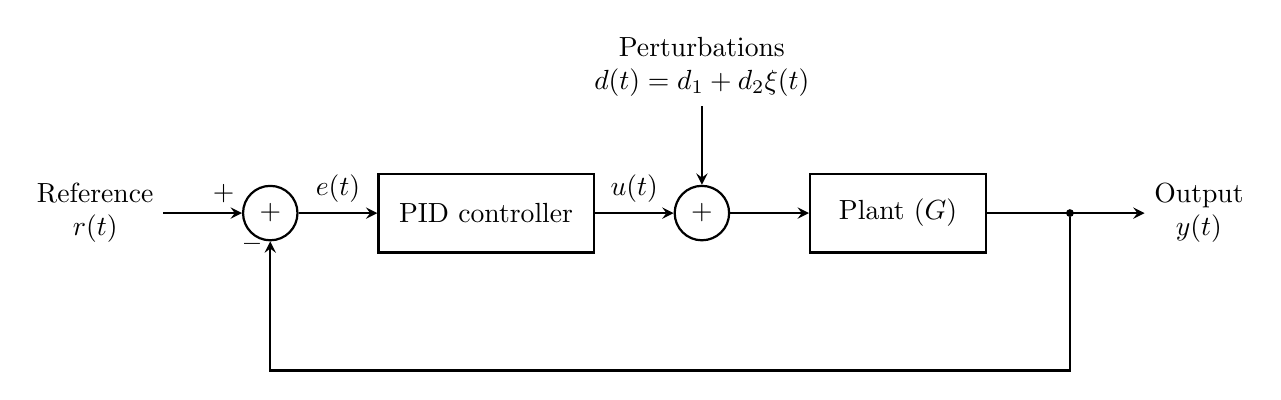
\begin{tikzpicture}[node distance = 10mm, auto]
	\node (Reference) [align=center] {Reference\\$r(t)$};
	\node (SummingPoint) [draw,circle, thick, right = of Reference]  {+};
	\node (Control) [block, text width = 2.5cm, right = of SummingPoint] {PID controller};
	\node (SummingPoint1) [draw,circle, thick, right = of Control]  {+};
	\node (Plant) [block, text width = 2cm, right = of SummingPoint1] {Plant ($G$)};
	\node (PlantRight) [support, right = of Plant, right = 1cm, fill, circle,scale=0.3] {};
	\node (Output) [right = of Plant, right = 2cm, align=center] {Output\\$y(t)$};
	\node (Perturbations) [align=center, above = of SummingPoint1] {Perturbations\\$d(t)=d_1+d_2\xi(t)$};
	\draw [arrow] (Reference) -- node[anchor=south west]{+}(SummingPoint);
	\draw [arrow] (SummingPoint) -- node[anchor=south]{$e(t)$}(Control);
	\draw [arrow] (Control) -- node[anchor=south]{$u(t)$}(SummingPoint1);
	\draw [arrow] (SummingPoint1) -- (Plant);
	\draw [arrow] (Plant) -- (Output);
	\draw [arrow] (PlantRight) -- +(0, -2) -| (SummingPoint) node[below = 2mm, anchor=north east]{\bf\textendash};
	\draw [arrow] (Perturbations) -- (SummingPoint1);
	\end{tikzpicture}
	\caption{Closed loop system with a PID Controller}
	\label{Fig:BlockDiagramPID}
\end{figure}

\begin{figure}
	\centering
	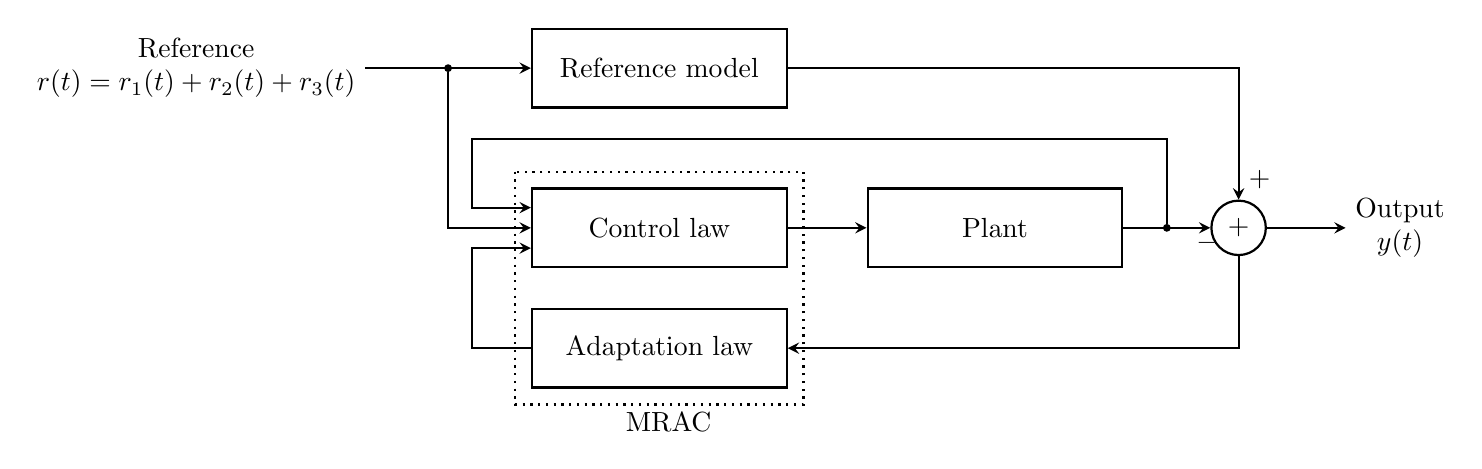
\begin{tikzpicture}[node distance = 10mm, auto]
	\node (Reference) [align=center] {Reference\\$r(t)=r_1(t)+r_2(t)+r_3(t)$};
	\node (ReferenceRight) [support, right = of Reference, fill,circle,scale=0.3] {};
	\node (RefModel) [block, text width = 3cm, right = of ReferenceRight] {Reference model};
	\node (Control) [block, text width = 3cm, below = of RefModel] {Control law};
	\node (Adaptation) [block, text width = 3cm, below = of Control, below = 5mm] {Adaptation law};
	\draw[thick, dotted] ($(Control.north west)+(-0.2,0.2)$)  rectangle ($(Adaptation.south east)+(0.2,-0.2)$)  (60mm, -45mm) node[]{MRAC};
	\node (Plant) [block, text width = 3cm, right = of Control] {Plant};
	\node (PlantRight) [support, right = of Plant, right = 5mm, fill,circle,scale=0.3] {};
	\node (SummingPoint) [draw,circle, thick, right = of PlantRight, right = 5mm ]  {+};
	\node (Output) [right = of SummingPoint, align=center] {Output\\$y(t)$};
	
	\path (Reference.east) -- (Reference.east) coordinate[pos=05] (Reference1);
	\path (Control.west) -- (Control.north west) coordinate[pos=-0.5] (Control1);
	\path (Control.west) -- (Control.north west) coordinate[pos=+0.5] (Control2);
	
	\draw [arrow] (Reference) -- node[anchor=south west]{}(RefModel);
	\draw [arrow] (ReferenceRight) |- (Control);
	\draw [arrow] (RefModel) -| node[pos=0.85, anchor = north west]{+}(SummingPoint);
	\draw [arrow] (Control) -- (Plant);
	\draw [arrow] (Plant) -- node[pos=0.75, anchor=north west]{\bf\textendash}
	(SummingPoint);
	\draw [arrow] (SummingPoint) -- (Output);
	\draw [arrow] (SummingPoint) |- (Adaptation);
	\draw [arrow] (Adaptation) -| (35mm,-30mm) |- (Control1);
	\draw [arrow] (PlantRight) |- (35mm,-9mm) |- (Control2);
		\end{tikzpicture}
	\caption{Adaptive control}
	\label{Fig:BloackDiagramAdaptiveControl}
\end{figure}

\end{document}